\subsubsection{Descripci\'on} 
Dados un conjunto de atributos \(M\) y un sistema implicacional \(\Sigma\) sobre M, este algoritmo calcula los generadores minimales haciendo uso del concepto de \textit{Labeled Closed Set}, que se basa en que si tenemos un conjunto \(A \subseteq M\), \(A\) es generador minimal si \(X^+_{\Sigma} = A^+_{\Sigma}\) implica que \(X = A\) para todo  \(X \subseteq A\). 

Podemos definir el conjunto de \textit{Labeled Closed Sets} con respecto a \(\Sigma\) como:
\begin{center}
    \(\{<C,mg(C)> | \ C \subseteq M, \ C^+_{\Sigma} = C \}\)\\
    donde \(mg(C) = \{D \subseteq M \ | \ D \ es \ generador \ minimal \ y \ D^+_{\Sigma} = C \}\)
\end{center}

De esta forma, al calcular el conjunto de \textit{Labeled Closed Sets} con el siguiente algoritmo, autom\'aticamente se calculan los generadores minimales.

\subsubsection{C\'odigo} 
\lstinputlisting{r_code/labeled.closed.set.R}
\subsubsection{Ejemplo} 
A continuaci\'on se muestra un peque\~no ejemplo de ejecuci\'on del algoritmo. Para ello se parte del conjunto de atributos \(M\) y del conjunto de implicaciones \(\Gamma\) que se puede ver en la imagen \ref{fig:lcs_4}.
\begin{figure}[H]
    \centering
    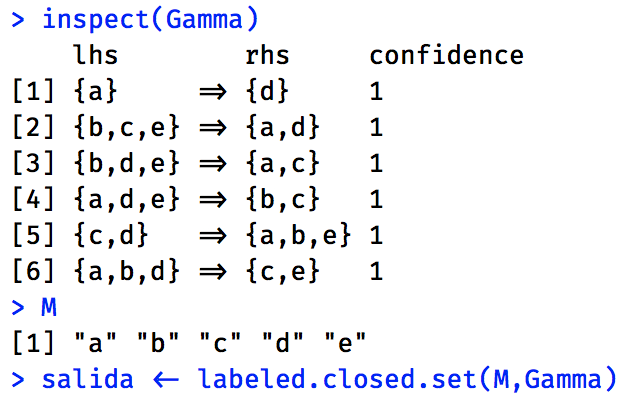
\includegraphics[scale=0.75]{lcs_4}
    \caption{Ejemplo LCS 1}
    \label{fig:lcs_4}
\end{figure} 
Aqu\'i se puede ver el resultado:
\begin{figure}[H]
    \centering
    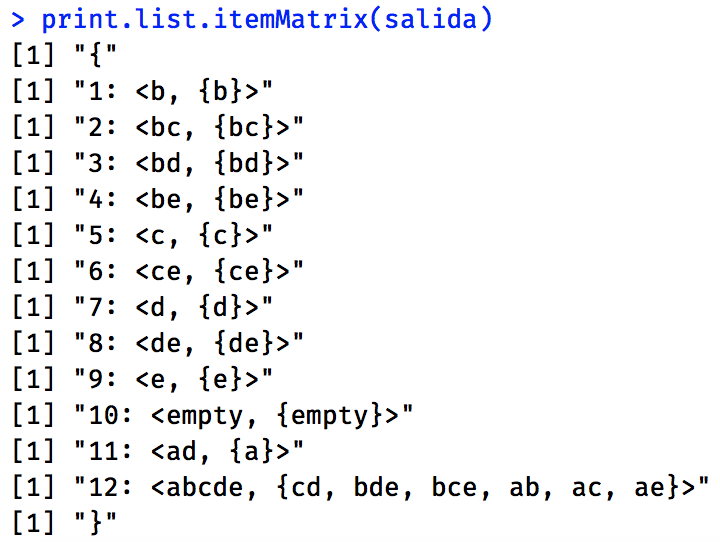
\includegraphics[scale=0.75]{lcs_3}
    \caption{Ejemplo LCS 2}
    \label{fig:lcs_3}
\end{figure}
Y aqu\'i el resultado que se obtendr\'ia si usamos la otra versi\'on del algoritmo:
\begin{figure}[H]
    \centering
    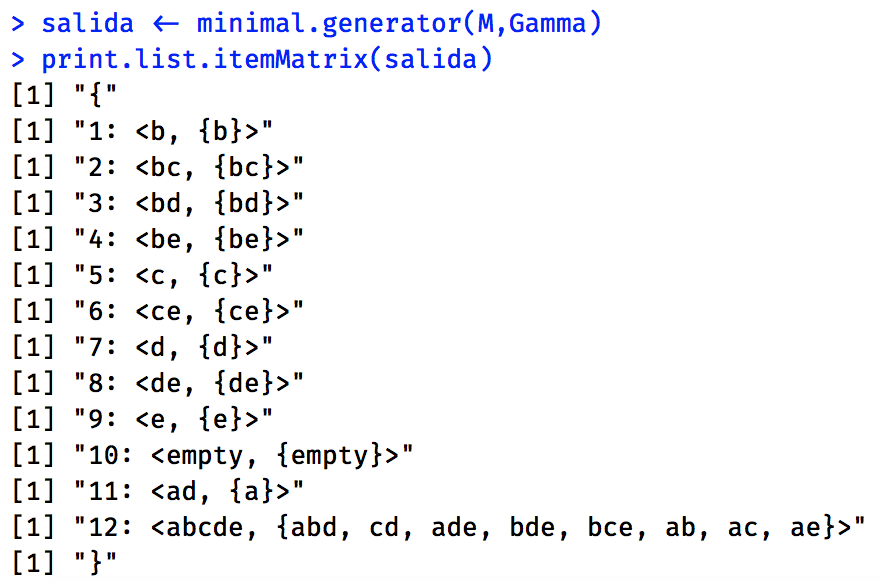
\includegraphics[scale=0.75]{lcs_5}
    \caption{Ejemplo LCS 3}
    \label{fig:lcs_5}
\end{figure}
\subsubsection{Comparativa/Versiones} 